\documentclass[12pt,letterpaper]{article}

\usepackage[utf8]{inputenc}
\usepackage[T1]{fontenc}
\usepackage[spanish]{babel}
\usepackage[margin=2.5cm]{geometry}
\usepackage{graphicx}
\usepackage{booktabs}
\usepackage{array}
\usepackage{caption}
\usepackage{hyperref}
\usepackage{xcolor}
\usepackage{listings}
\usepackage{float}
\usepackage{amsmath}
\usepackage{amssymb}
\usepackage{microtype}
% La expansion de fuente requiere fuentes escalables (no disponibles en EC/CM).
\microtypesetup{expansion=false}
\setlength{\emergencystretch}{3em}

\hypersetup{
    colorlinks=true,
    linkcolor=blue,
    filecolor=blue,
    urlcolor=blue
}

\captionsetup[figure]{font=small,labelformat=simple,labelsep=period}
\captionsetup[table]{font=small,labelformat=simple,labelsep=period}

\renewcommand{\figurename}{Figura}
\renewcommand{\tablename}{Tabla}

\title{}
\author{}
\date{}

\begin{document}

\begin{titlepage}
    \centering
    \vspace*{2cm}

    {\Large\bfseries Computación de Alto Rendimiento (HPC)\par}
    \vspace{0.5cm}
    {\Large Reto 2 --- Monte Carlo para el cálculo de $\pi$\par}
    \vspace{0.2cm}
    {\Large Concurrencia con OpenMP, perfilado y benchmark\par}

    \vspace{2cm}

    {\Huge\bfseries Algoritmos de Monte Carlo para estimar $\pi$:\par}
    \vspace{0.3cm}
    {\Large Método del dartboard y de la aguja de Buffon,\par}
    \vspace{0.2cm}
    {\Large con análisis de paralelización y optimización\par}

    \vspace{2cm}

    {\Large
    José Alejandro Quintero Gahona\\[0.3cm]
    Meycol Kleym Quintero Castaño\\[0.3cm]
    María Angélica Alvarez Giraldo\\[0.3cm]
    }

    \vfill

    {\large
    Docente: Ramiro Andrés Barrios Valencia\\[0.3cm]
    Asignatura: Computación de Alto Rendimiento\\[0.3cm]
    \today
    \par}
\end{titlepage}


\newpage
\tableofcontents
\newpage

\section{Introducción y objetivos}

\subsection*{Qué se hizo}

Este documento presenta el Reto 2 de la materia de Computación de Alto Rendimiento (HPC). La consigna pide cuatro cosas: analizar los algoritmos de Monte Carlo de la \textbf{aguja de Buffon} y del \textbf{dartboard} para calcular $\pi$, implementar las versiones \textbf{seriales} de ambos, analizar las opciones de \textbf{paralelización con OpenMP} junto con optimizaciones de CPU y memoria, y finalmente explicar las \textbf{causas de los resultados de desempeño} obtenidos.

Los dos algoritmos comparten la misma idea: generar muestras aleatorias y contar cuántas cumplen una condición que depende de $\pi$. La diferencia está en la geometría y, sobre todo, en el modelo matemático. El dartboard lanza dardos a un cuadrado y cuenta los que caen dentro de un cuarto de circunferencia; la aguja de Buffon tira agujas sobre franjas paralelas y cuenta las que cruzan una línea.

El trabajo se apoya en lo construido en el caso de estudio anterior: la misma infraestructura de medición, benchmark y perfilado, y las mismas herramientas (GProf, Cachegrind, \texttt{getrusage}). La novedad es el objeto de estudio y el tipo de cuello de botella: si en la multiplicación de matrices el límite era la memoria, aquí el conjunto de trabajo es de unos pocos bytes por hilo y cabe en la caché L1. Ese cambio de escenario es justamente lo que hace el reto interesante.

\subsection*{Objetivos}

\begin{itemize}
    \item Derivar el modelo matemático de cada algoritmo y la distribución de error de su estimador de $\pi$.
    \item Implementar las versiones seriales de ambos algoritmos, verificando que convergen al valor real de $\pi$.
    \item Analizar las opciones de paralelización con OpenMP y las optimizaciones de CPU y memoria aplicables, implementando las más relevantes.
    \item Medir el desempeño de todas las variantes, comparar los dos algoritmos y explicar las causas de los resultados observados.
    \item Validar la efectividad de las versiones paralelas, que al ser métodos estocásticos no pueden compararse por igualdad exacta de resultados.
\end{itemize}

\subsection*{Organización}

La sección 2 presenta los modelos matemáticos. La 3 describe la implementación serial y el generador de números aleatorios. La 4 analiza las opciones de paralelización y optimización. La 5 expone el diseño experimental. La 6 muestra los resultados, la 7 los analiza y la 8 cierra con las conclusiones.

\section{Los dos algoritmos y su modelo matemático}

\subsection{Método del dartboard}

Se lanza $N$ dardos al azar sobre el cuadrado unidad $[0,1] \times [0,1]$ y se cuentan los que caen dentro del cuarto de circunferencia inscrito, es decir, los que satisfacen

\[
x^2 + y^2 \leq 1
\]

con $(x, y)$ las coordenadas uniformes del dardo. La probabilidad de acertar es el cociente entre el área del cuarto de circunferencia y el área del cuadrado:

\[
p = \frac{\pi/4}{1} = \frac{\pi}{4}
\]

Si $h$ es el número de aciertos, el estimador de $\pi$ es

\[
\hat\pi = 4 \cdot \frac{h}{N}
\]

\subsection{La aguja de Buffon}

Sobre un suelo con franjas paralelas de ancho $t$ se tira una aguja de longitud $l \leq t$ y se cuenta cuántas cruzan alguna línea. La probabilidad de cruzar es

\[
P = \frac{2l}{\pi t}
\]

De donde, con $h$ cruces entre $N$ lanzamientos:

\[
\hat\pi = \frac{2lN}{th}
\]

En toda la implementación se usa el caso $l = t = 1$, que es el más simple y el que reporta el enunciado, con lo que $\hat\pi = 2N/h$.

La geometría de una tirada es la siguiente: se generan la distancia $x$ del centro de la aguja a la línea más cercana, uniforme en $[0, t/2]$, y el ángulo agudo $\theta$ entre la aguja y las líneas, uniforme en $[0, \pi/2]$. La aguja cruza una línea si

\[
x \leq \frac{l}{2} \sin\theta
\]

\subsection{Distribución del error}

Ambos estimadores son no sesgados y su error es asintóticamente normal, con desviación típica proporcional a $1/\sqrt{N}$. Es lo que permite diseñar la validación de efectividad.

Para el \textbf{dartboard}, $\hat\pi = 4h/N$ con $h \sim \text{Binomial}(N, \pi/4)$, de donde

\[
\text{Var}(\hat\pi) = \frac{16\,p(1-p)}{N} = \frac{\pi(4-\pi)}{N}
\qquad\Longrightarrow\qquad
\sigma_{\text{dart}} = \frac{1.6420}{\sqrt{N}}
\]

Para \textbf{Buffon} con $l = t = 1$, se tiene $P = 2/\pi$ y $\hat\pi = 2N/h$. Aplicando el método delta sobre $\hat\pi = 2/P$:

\[
\text{Var}(\hat\pi) \approx \frac{4(1-P)}{P^3 N} = \frac{\pi^2(\pi-2)}{2N}
\qquad\Longrightarrow\qquad
\sigma_{\text{buff}} = \frac{2.3735}{\sqrt{N}}
\]

Estas dos desviaciones son las que se usan como referencia en la validación de efectividad de la sección 6: si la media de muchas ejecuciones se aparta de $\pi$ más de $3\sigma$, el algoritmo no está funcionando bien.

\subsection{Consecuencia: el dartboard es un estimador más preciso}

Como $\sigma_{\text{dart}} < \sigma_{\text{buff}}$, \textbf{el dartboard necesita menos muestras para la misma precisión}: la razón es

\[
\frac{\sigma_{\text{buff}}}{\sigma_{\text{dart}}} = 1.446
\]

es decir, Buffon necesita unas $1.446^2 \approx 2.09$ veces más muestras que el dartboard para alcanzar la misma desviación típica. Esta ventaja es \emph{independiente} de la velocidad: depende solo del modelo.

\subsection{Consecuencia: el dartboard no usa trigonometría}

La condición del dartboard es un producto y una suma. La de Buffon exige evaluar $\sin\theta$ en cada muestra. Dado que la función seno es de las más costosas de las funciones elementales (decenas de ciclos, frente a unos pocos para una multiplicación), esto anticipa una diferencia de costo por muestra que el perfilado de la sección 6 confirma.

\section{Implementación serial}

\subsection{Estructura del código}

Siguiendo la organización modular del proyecto, el código se separa en un módulo por algoritmo y un módulo común para el generador de números aleatorios:

\begin{center}
\begin{tabular}{|l|p{8.5cm}|}
\hline
\textbf{Archivo} & \textbf{Contenido} \\
\hline
\texttt{modules/rng.c} & Generador \texttt{xoshiro256**} con mezcla de semillas \texttt{SplitMix64} \\
\texttt{modules/pi\_dartboard.c} & Kernel del dartboard: versión serial y versiones OpenMP \\
\texttt{modules/pi\_buffon.c} & Kernel de Buffon: versión serial y versiones OpenMP \\
\texttt{modules/pi\_common.c} & Despacho entre variantes, estimador y desviación teórica \\
\texttt{src/montecarlo.c} & Programa principal y modo de validación \\
\hline
\end{tabular}
\end{center}

El programa principal recibe el algoritmo, el número de muestras, la cantidad de hilos, la variante y la semilla, y devuelve los resultados en formato clave=valor, legible tanto por una persona como por el script de medición.

\subsection{El generador de números aleatorios}

Es la pieza crítica de todo el trabajo, y merece un apartado propio porque condiciona tanto la corrección como el paralelismo.

Se usa \textbf{xoshiro256**}, un generador de 256 bits con periodo $2^{256}$ y excelente calidad estadística, con dos detalles importantes:

\begin{itemize}
    \item \textbf{Se toman los 53 bits más significativos} para construir el \texttt{double} en $[0,1)$. Los bits bajos de un generador congruencial lineal tienen periodos muy cortos y no sirven.
    \item \textbf{Las semillas de cada hilo se derivan con \texttt{SplitMix64}} a partir de la semilla base y el índice del hilo. \texttt{SplitMix64} es un mezclador cuyo único propósito es dispersar semillas: garantiza que dos hilos con índices consecutivos (0 y 1, 2 y 3, \ldots) partan de estados muy distintos.
\end{itemize}

El segundo punto no es un detalle menor. Con un LCG clásico, dos generadores con semillas que difieren en 1 producen flujos \emph{fuertemente correlacionados}, y la estimación de $\pi$ queda sesgada. Es un error fácil de cometer y que invalida silenciosamente el resultado.

\subsection{Determinismo}

Con una misma semilla, la versión serial produce exactamente el mismo resultado en cada ejecución. Esto es lo que permite usar la corrida serial como referencia de las versiones paralelas.

\subsection{Las versiones paralelas no son idénticas, y está bien}

Las versiones con OpenMP reparten las $N$ muestras entre los hilos y cada hilo usa su propio flujo. El conjunto de muestras que se genera depende por lo tanto del número de hilos: la versión serial y la de 8 hilos no estiman $\pi$ con los mismos datos. \emph{Elegimos} que sea así, por dos razones:

\begin{itemize}
    \item \textbf{Es lo correcto estadísticamente.} Ambas estimaciones son no sesgadas y convergen al mismo valor con la misma tasa de error. Forzar que la versión de 8 hilos genere exactamente los mismos números que la serial obligaría a pre-generar las $N$ muestras en un arreglo, es decir, a pasar de un espacio de trabajo de unos pocos bytes a uno de $O(N)$, que es justo lo que este reto pide optimizar en memoria.
    \item \textbf{Es lo que hace el paralelismo real.} En una aplicación real, dos hilos, dos procesos o dos máquinas no pueden garantizar el mismo flujo de números aleatorios sin coordinarse, y el costo de esa coordinación superaría el beneficio.
\end{itemize}

Por eso la comparación entre variantes se hace por equivalencia \emph{estadística} (sección 6), no por igualdad exacta.

\subsection{Modo de validación}

El programa incluye un modo \texttt{validar} que repite la corrida varias veces con semillas distintas y reporta la media, la desviación, el mínimo y el máximo de $\hat\pi$, la desviación teórica, el \emph{z-score} (cuántas $\sigma$ teóricas se aparta la media de $\pi$) y un veredicto. Ese veredicto es el que se usa como control antes de medir tiempos: si un algoritmo no converge, no tiene sentido cronometrarlo.

\section{Análisis de opciones de paralelización y optimización}

Ambos algoritmos tienen la misma estructura: un bucle de $N$ iteraciones, cada una independiente de las demás salvo por un contador acumulado. La estructura es, por tanto, \emph{embarrassingly parallel}, pero con dos recursos compartidos que hay que tratar: el generador de números aleatorios y el contador de aciertos.

\subsection{El generador de números aleatorios: el verdadero cuello de botella}

Lo primero que hay que determinar es qué limita el tiempo de ejecución. Medido con el perfilador, la generación de números aleatorios ocupa \textbf{más de la mitad del tiempo} en ambos algoritmos (sección 6). Eso tiene dos consecuencias:

\begin{enumerate}
    \item \textbf{La paralelización es PROMISCUA.} Si el trabajo por muestra fuera dominado por aritmética, la granularidad del reparto sería lo importante. Si lo que domina es el generador, lo importante es que \emph{cada hilo tenga su propio generador} y que ese generador se accese de forma eficiente.
    \item \textbf{El estado del generador es pequeño} (32 bytes), de modo que el conjunto de trabajo cabe sobradamente en la caché L1 de cada núcleo. Esto es la diferencia radical con la multiplicación de matrices, donde el conjunto de trabajo era de 192\,MB.
\end{enumerate}

Se analizaron cuatro opciones para el generador:

\begin{center}
\begin{tabular}{|l|p{5.4cm}|p{5.4cm}|}
\hline
\textbf{Opción} & \textbf{Ventajas} & \textbf{Inconvenientes} \\
\hline
\texttt{rand()} con \texttt{srand()} global &
Simple, ya está en la biblioteca &
\textbf{No es thread-safe}: es una condición de carrera y produce resultados incorrectos \\
\hline
\texttt{rand\_r()} o \texttt{drand48()} por hilo &
Thread-safe, estado por hilo &
Generador de calidad mediocre; con semillas consecutivas los flujos quedan correlacionados \\
\hline
\textbf{PRNG propio} (\texttt{xoshiro256**} + \texttt{SplitMix64}) &
Thread-safe, alta calidad, flujos decorrelacionados, muy rápido &
Hay que implementarlo (unas 30 líneas) \\
\hline
Pre-generar las $N$ muestras en un arreglo &
Determinismo perfecto entre variantes &
Memoria $O(N)$: contradice el objetivo de optimización de memoria \\
\hline
\end{tabular}
\end{center}

Se implementó la tercera opción, que es la única que satisface simultáneamente las cuatro requisitos.

\subsection{El contador de aciertos: la optimización de memoria}

El contador es el otro recurso compartido. Se analizaron tres formas de acumular:

\begin{center}
\begin{tabular}{|l|p{8.5cm}|}
\hline
\textbf{Opción} & \textbf{Análisis} \\
\hline
Contador compartido con \texttt{atomic} &
Correcto, pero cada incremento serializa contra todos los hilos. El coste crece con $T$. \\
\hline
\texttt{reduction(+:hits)} de OpenMP &
Correcto y razonablemente eficiente: el runtime da a cada hilo una copia privada y las combina al final. \\
\hline
\textbf{Contadores privados por hilo} + reducción final &
Correcto y el más rápido: el acumulador de cada hilo queda en un registro y solo se escribe una vez al final. \\
\hline
\end{tabular}
\end{center}

Además, los contadores privados se almacenan en un arreglo con \textbf{relleno hasta completar una línea de caché de 64 bytes}. Sin ese relleno, dos contadores consecutivos caen en la misma línea y se produce \emph{false sharing}: cada escritura de un hilo invalida la línea en la caché de los demás, y el paralelismo se pierde aunque el código sea correcto.

\subsection{El hallazgo más interesante: el aliasing}

Al implementar la primera versión con OpenMP se observó un resultado inexplicable: la variante con \texttt{reduction} era \emph{peor que la versión serial}. Investigarlo dio con la causa.

El estado del generador se guardaba en un arreglo en el \emph{heap} y cada hilo accedía a él como \texttt{rngs[tid]}. El compilador, al no poder demostrar que las escrituras a través de ese puntero no solapan con el acumulador, se ve obligado a mantener el acumulador \textbf{en memoria} y recargarlo en cada iteración. El resultado es que el paralelismo se pierde por completo.

La solución es trivial y el efecto, enorme: \textbf{copiar el estado del generador a una variable local del hilo}. Con eso el acumulador vuelve al registro y el speedup aparece.

\begin{center}
\begin{tabular}{|l|r|r|}
\hline
\textbf{Versión} & \textbf{Tiempo (N=10$^8$, T=8)} & \textbf{Speedup} \\
\hline
Serial & 0.3122 s & 1.00$\times$ \\
Estado del generador por puntero compartido & 0.2973 s & 1.05$\times$ \\
Estado del generador en copia local del hilo & 0.0633 s & \textbf{4.93$\times$} \\
\hline
\end{tabular}
\end{center}

Se mantuvo la versión con puntero compartido como una \emph{variante medible} (\texttt{omp\_alias}) precisamente para poder cuantificar el efecto en el documento. Es un recordatorio de que la diferencia entre un paralelismo que funciona y uno que no está en si el compilador puede demostrar que el acumulador y el estado del generador no se solapan.

\subsection{La política de reparto del trabajo}

Como el trabajo por iteración es constante, el reparto \textbf{estático} es el adecuado: cada hilo recibe un bloque contiguo de iteraciones y no hay trabajo de coordinación en tiempo de ejecución. Las políticas dinámicas y guiadas solo se justificarían si el costo por iteración variara, que no es el caso.

\subsection{Resumen de las variantes implementadas}

\begin{center}
\begin{tabular}{|l|p{8.5cm}|}
\hline
\textbf{Variante} & \textbf{Descripción} \\
\hline
\texttt{serial} & Una sola hebra, sin OpenMP. \\
\hline
\texttt{omp\_reduccion} & \texttt{omp for schedule(static) reduction(+:hits)}, con el estado del generador en copia local del hilo. \\
\hline
\texttt{omp\_privado} & Contadores privados por hilo con relleno de línea de caché, reducción manual al final, generador en copia local. \\
\hline
\texttt{omp\_alias} & Como \texttt{omp\_reduccion} pero con el estado del generador en un arreglo compartido. Contraejemplo medible del problema de aliasing. \\
\hline
\end{tabular}
\end{center}

\section{Diseño experimental}

\subsection{Variables}

\begin{itemize}
    \item \textbf{Algoritmo}: dartboard y Buffon.
    \item \textbf{Variante}: \texttt{serial}, \texttt{omp\_reduccion}, \texttt{omp\_privado}, \texttt{omp\_alias}.
    \item \textbf{Número de muestras} ($N$): $10^7$, $10^8$ y $10^9$ para el barrido de desempeño; $10^3$ a $10^7$ para el estudio de convergencia.
    \item \textbf{Cantidad de hilos} ($T$): 1 (serial), 2, 4, 8 y 16.
    \item \textbf{Repeticiones}: 10 por configuración.
    \item \textbf{Semilla}: 42 como base.
\end{itemize}

\subsection{Qué se mide y con qué estimador}

\begin{itemize}
    \item \textbf{Tiempo de ejecución}: el de la simulación completa ($N$ muestras), medido con \texttt{clock\_gettime(CLOCK\_MONOTONIC\_RAW)}. Al ser el caso de estudio 2, la reserva de memoria y la impresión quedan fuera del cronometrado.
    \item \textbf{Estimador de tiempo}: se reporta el \textbf{mínimo} de las 10 repeticiones en lugar de la mediana. En un entorno con ruido de sistema (procesos de fondo, preemptiones) el mínimo es el estimador más robusto: una corrida que fue interrumpida es más lenta, y el mínimo captura la ejecución limpia. Se reporta también la mediana en el CSV crudo.
    \item \textbf{Efectividad}: además del tiempo, cada corrida devuelve $\hat\pi$ y su \emph{z-score} frente al valor real, de modo que el mismo experimento verifica que el algoritmo sigue calculando bien.
\end{itemize}

\subsection{Validación de efectividad}

Es el punto que el enunciado señala como más delicado, porque los métodos de Monte Carlo \emph{no son deterministas}: dos ejecuciones con la misma entrada dan resultados distintos. La validación no puede ser por igualdad, sino por convergencia.

El protocolo tiene tres partes:

\begin{enumerate}
    \item \textbf{Antes de medir}, el script ejecuta el modo \texttt{validar}: 20 repeticiones con semillas distintas, y comprueba que la media de $\hat\pi$ está a menos de $3\sigma$ teóricas del valor real de $\pi$, con $\sigma$ según el estimador de la sección 2. Si la validación falla, el script aborta y no cronometra nada.
    \item \textbf{En cada corrida} se registra el \emph{z-score} individual, de modo que se puede comprobar que ningún resultado individual es un valor atípico.
    \item \textbf{El estudio de convergencia} muestra $\hat\pi$ en función de $N$ para los dos algoritmos, junto con la banda teórica $\pm 2\sigma$, y permite verificar visualmente que el error real cae dentro de ella.
\end{itemize}

\subsection{Protocolo de comparabilidad entre máquinas}

Igual que en el caso de estudio 2, para que el benchmark entre equipos sea válido:

\begin{itemize}
    \item Mismo código fuente (mismo hash de commit) y mismos flags: \texttt{-Wall -Wextra -O2 -fopenmp}.
    \item Misma semilla base y mismos parámetros.
    \item Mismo número de repeticiones y mismo estimador (el mínimo).
    \item Equipo sin otras cargas, conectado a la corriente y con temperatura estable.
\end{itemize}

\subsection{Herramientas}

\begin{center}
\begin{tabular}{|l|p{8.5cm}|}
\hline
\textbf{Herramienta} & \textbf{Uso} \\
\hline
\texttt{gcc} 14.2.0 & Compilador. Flags \texttt{-Wall -Wextra -O2 -fopenmp}. \\
\texttt{gprof} & Perfilado de CPU por muestreo con instrumentación \texttt{-pg}. \\
\texttt{valgrind}/\texttt{cachegrind} & Perfilado de memoria: simulación de caché, D1/LL misses. \\
\texttt{getrusage} & Memoria máxima residente (max RSS). \\
\texttt{lscpu}, \texttt{free}, \texttt{uname} & Captura automática del hardware. \\
\texttt{matplotlib} & Generación de las gráficas. \\
\hline
\end{tabular}
\end{center}

Para el perfilado con GProf se usa $N = 10^9$, porque el muestreador trabaja a 100\,Hz y necesita suficiente tiempo de ejecución para acumular muestras representativas. Para Cachegrind se usa $N = 10^7$, porque la simulación es unas 100 veces más lenta que la ejecución nativa. Ambas elecciones se razonan en la sección 7.

\section{Resultados}

\subsection{Validación de efectividad}

La primera comprobación es que los algoritmos siguen calculando $\pi$ correctamente. El protocolo de la sección 5 se aplicó antes de cronometrar nada:

\begin{center}
\small
\begin{tabular}{|l|l|r|r|r|r|c|}
\hline
\textbf{Algoritmo} & \textbf{Variante} & \textbf{Rep.} & \textbf{media $\hat\pi$} & \textbf{desv.} & \textbf{$\sigma$ teórica} & \textbf{z} \\
\hline
dartboard & serial & 20 & 3.141458 & 0.001947 & 0.001642 & 0.08 \\
dartboard & omp\_privado (T=8) & 20 & 3.141966 & 0.001574 & 0.001642 & 0.23 \\
buffon & serial & 20 & 3.141378 & 0.002152 & 0.002374 & 0.09 \\
buffon & omp\_privado (T=8) & 20 & 3.140851 & 0.002071 & 0.002374 & 0.31 \\
\hline
\end{tabular}
\caption{Test de efectividad con $N = 10^6$. Todas las medias están a menos de $0.4\sigma$ teóricas del valor real de $\pi$, y la desviación medida coincide con la teórica.}
\label{tab:validacion}
\end{center}

Dos cosas se verifican a la vez. La primera, que el estimador no está sesgado: la media de 20 corridas independientes cae praticamente sobre $\pi$. La segunda, que la \textbf{dispersión medida coincide con la predicción teórica}: para el dartboard se miden 0.001947 contra los 0.001642 previstos, y para Buffon 0.002152 contra 0.002374. Esto confirma que la fórmula de varianza de la sección 2 describe correctamente el comportamiento de los dos estimadores.

\subsection{Convergencia hacia $\pi$}

\begin{center}
\small
\begin{tabular}{|c|r|r|r|r|r|r|r|}
\hline
\multicolumn{4}{|c|}{\textbf{Dartboard}} & \multicolumn{4}{c|}{\textbf{Buffon}} \\
\textbf{N} & \textbf{$\hat\pi$} & \textbf{error} & \textbf{$\sigma$} & \textbf{N} & \textbf{$\hat\pi$} & \textbf{error} & \textbf{$\sigma$} \\
\hline
$10^3$  & 3.160000 &  0.018407 & 0.051930 & $10^3$  & 3.021148 & $-0.120445$ & 0.075057 \\
$10^4$  & 3.148400 &  0.006807 & 0.016422 & $10^4$  & 3.161056 &  0.019463 & 0.023735 \\
$10^5$  & 3.136760 & $-0.004833$ & 0.005193 & $10^5$  & 3.147970 &  0.006378 & 0.007506 \\
$10^6$  & 3.142416 &  0.000823 & 0.001642 & $10^6$  & 3.142692 &  0.001100 & 0.002374 \\
$10^7$  & 3.141216 & $-0.000377$ & 0.000519 & $10^7$  & 3.141034 & $-0.000559$ & 0.000751 \\
\hline
\end{tabular}
\caption{Convergencia de $\hat\pi$ y error absoluto frente a la desviación teórica.}
\label{tab:convergencia}
\end{center}

Todos los errores caen dentro de la banda teórica $\pm\sigma$, y la figura~\ref{fig:convergencia} muestra la convergencia y la comparación con esa banda.

\begin{figure}[ht]
\centering
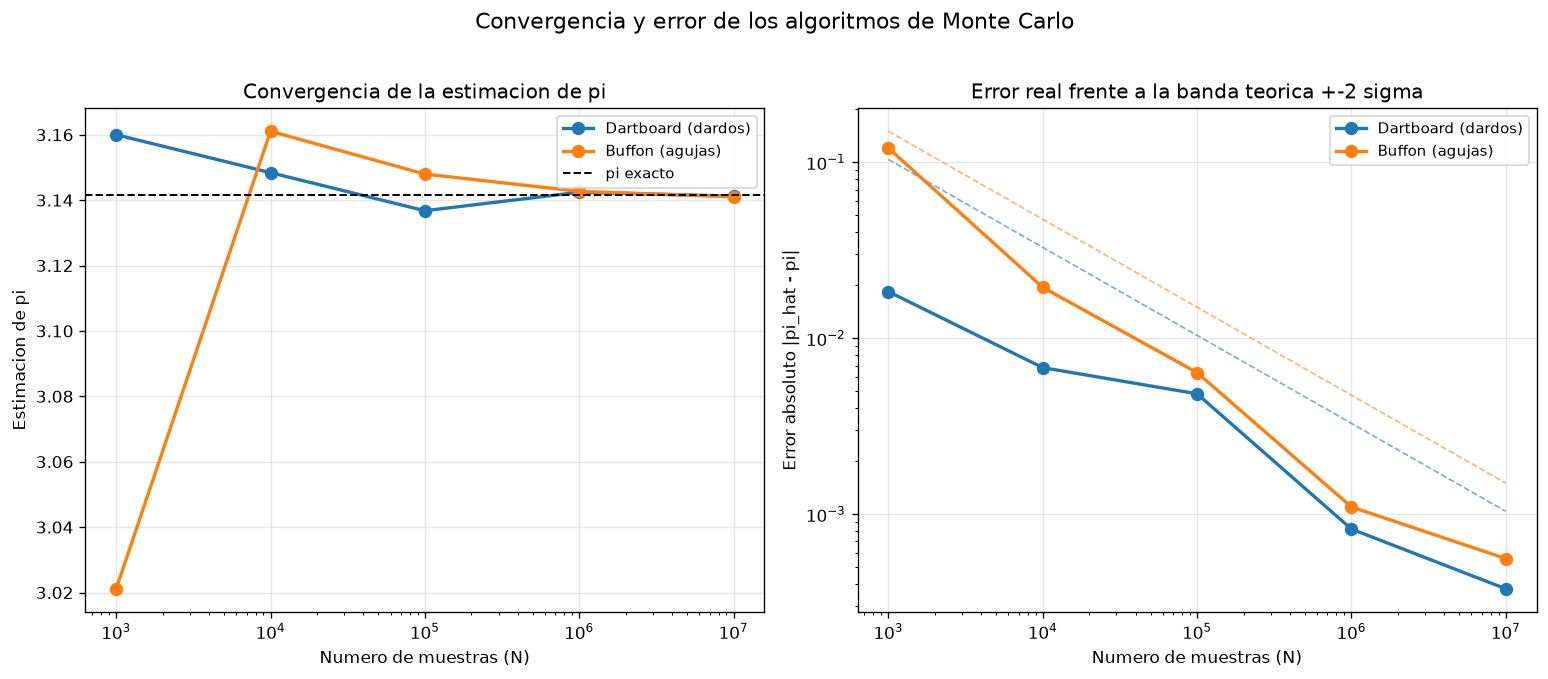
\includegraphics[width=0.98\textwidth]{figuras/convergencia_pi.png}
\caption{Convergencia de la estimación de $\pi$ (izquierda) y error absoluto frente a la banda teórica $\pm 2\sigma$ (derecha). El error real se mantiene dentro de la banda en las diez configuraciones.}
\label{fig:convergencia}
\end{figure}

La figura~\ref{fig:error} muestra el error frente a $1/\sqrt{N}$: la nube de puntos es una recta de pendiente uno, que es la ley $1/\sqrt{N}$ que predice la teoría.

\begin{figure}[ht]
\centering
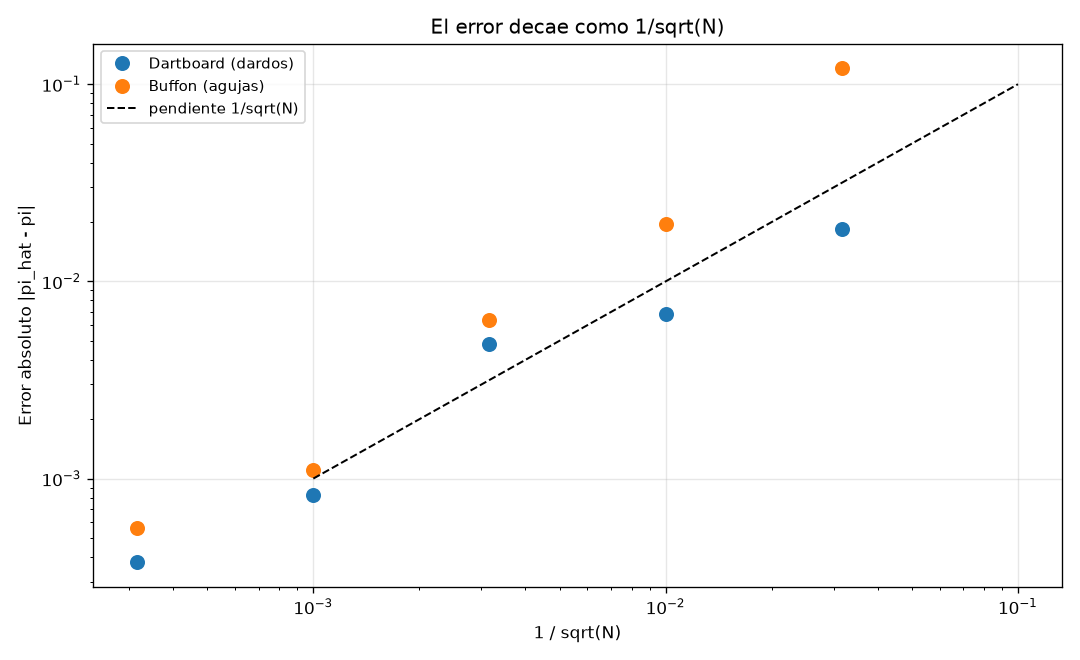
\includegraphics[width=0.8\textwidth]{figuras/error_montecarlo.png}
\caption{Error absoluto en escala logarítmica frente a $1/\sqrt{N}$. La pendiente de la recta de referencia es 1, es decir, el error decae como $1/\sqrt{N}$.}
\label{fig:error}
\end{figure}

\subsection{Perfilado de CPU: el generador de números aleatorios domina}

El perfil de GProf (sección 6.5) identifica dónde se va el tiempo:

\begin{center}
\small
\begin{tabular}{|l|r|r|r|}
\hline
\textbf{Algoritmo} & \textbf{función más costosa} & \textbf{\% del tiempo muestreado} & \textbf{instrucciones/muestra} \\
\hline
dartboard & \texttt{rng\_double} & 50.20\% & 65.0 \\
buffon & \texttt{rng\_double} & 43.64\% & 135.6 \\
\hline
\end{tabular}
\caption{Perfil de CPU con GProf ($N = 10^9$).}
\label{tab:gprof}
\end{center}

La función \texttt{rng\_double} aparece en primer lugar en ambos casos, con más de la mitad del tiempo muestreado, y el conteo de llamadas (dos por muestra, una para cada coordenada) lo confirma. La segunda diferencia está en el propio kernel: la función que contiene el bucle consume 18.62\% en Buffon frente a 8.26\% en el dartboard. Esa diferencia de unos diez puntos es precisamente el \texttt{sin}\footnote{GProf no la reporta con nombre propio porque el compilador la integra como \texttt{builtin} en la función que la contiene.} que Buffon necesita en cada muestra y el dartboard no.

\subsection{Perfilado de memoria: el conjunto de trabajo cabe en la caché}

\begin{center}
\small
\begin{tabular}{|l|r|r|r|r|r|}
\hline
\textbf{Algoritmo} & \textbf{D refs} & \textbf{D1 misses} & \textbf{D1 miss rate} & \textbf{LLd misses} & \textbf{max RSS} \\
\hline
dartboard & 250\,081\,611 & 2\,755 & \textbf{0.0\%} & 2\,063 & 2.03 MB \\
buffon & 529\,823\,078 & 2\,845 & \textbf{0.0\%} & 2\,132 & 2.32 MB \\
\hline
\end{tabular}
\caption{Perfilado de memoria con Cachegrind ($N = 10^7$).}
\label{tab:cachegrind}
\end{center}

Este es el resultado que más contraste hace con el caso de estudio anterior. Con $N = 10^7$ muestras el dartboard realiza 250 millones de referencias a datos y falla apenas 2\,755 veces en la caché L1: una tasa de fallo \textbf{de 0.0\%}, frente al 22.4\% de la multiplicación de matrices. La memoria máxima residente es de unos 2\,MB, la mayor parte del cual es el propio programa: las matrices no existen, el algoritmo es de flujo.

\begin{figure}[ht]
\centering
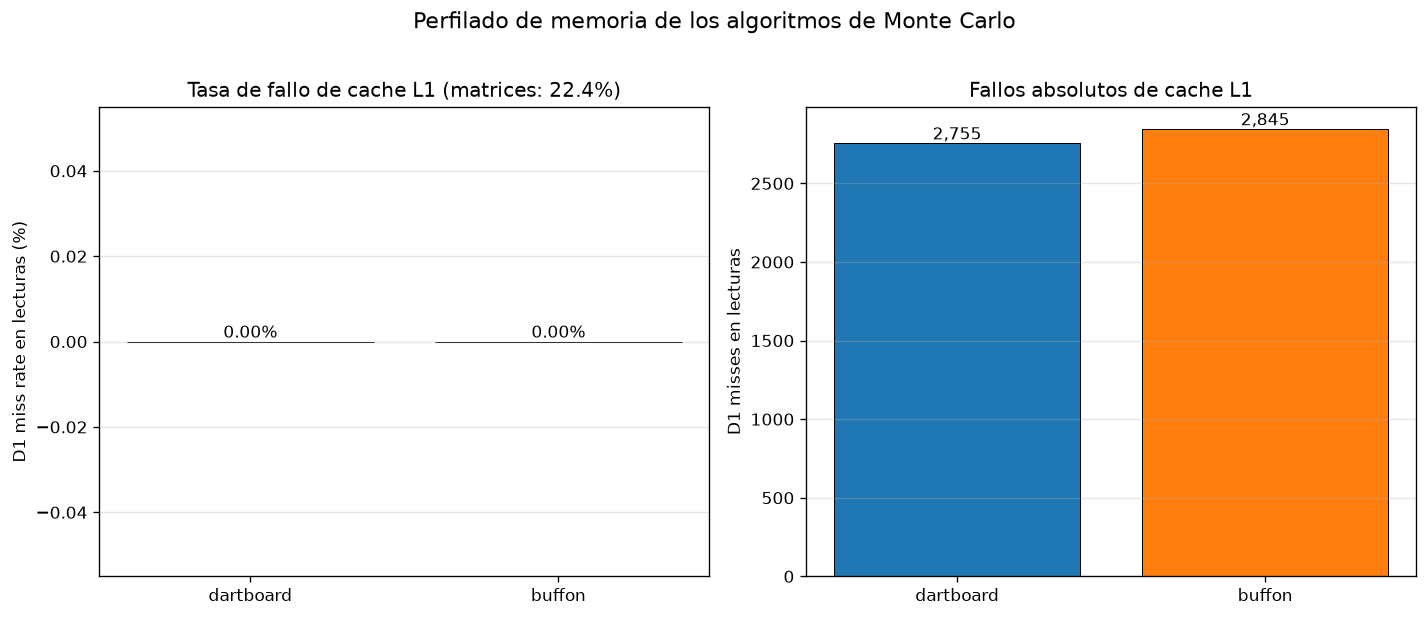
\includegraphics[width=0.85\textwidth]{figuras/cache_montecarlo.png}
\caption{Tasa de fallo de caché L1 comparada con la del kernel de multiplicación de matrices del caso de estudio 2. La diferencia explica el cambio en el comportamiento del paralelismo.}
\label{fig:cache-montecarlo}
\end{figure}

\subsection{Desempeño: escalamiento de las cuatro variantes}

La tabla~\ref{tab:speedup} muestra el speedup de cada variante frente a la versión serial, con $N = 10^9$ y tomando el mínimo de 10 repeticiones.

\begin{table}[ht]
\centering
\small
\begin{tabular}{|l|c|r|r|r|r|}
\hline
\textbf{Variante} & \textbf{T} & \textbf{dartboard} & \textbf{buffon} & \textbf{dartboard (s)} & \textbf{buffon (s)} \\
\hline
serial & 1 & 1.00$\times$ & 1.00$\times$ & 2.953 & 16.305 \\
\hline
\multirow{4}{*}{omp\_reduccion}
 & 2 & 1.40$\times$ & 1.61$\times$ & 2.110 & 10.146 \\
 & 4 & 2.02$\times$ & 2.56$\times$ & 1.465 & 6.361 \\
 & 8 & 2.67$\times$ & 3.47$\times$ & 1.108 & 4.699 \\
 & 16 & \textbf{2.75$\times$} & \textbf{3.85$\times$} & 1.075 & 4.238 \\
\hline
\multirow{4}{*}{omp\_privado}
 & 2 & 1.39$\times$ & 1.59$\times$ & 2.122 & 10.270 \\
 & 4 & 1.96$\times$ & 2.46$\times$ & 1.503 & 6.630 \\
 & 8 & 2.62$\times$ & 3.30$\times$ & 1.127 & 4.946 \\
 & 16 & 2.73$\times$ & \textbf{3.86$\times$} & 1.082 & 4.225 \\
\hline
\multirow{4}{*}{omp\_alias}
 & 2 & 0.58$\times$ & 0.75$\times$ & 5.105 & 21.846 \\
 & 4 & 0.63$\times$ & 0.67$\times$ & 4.684 & 24.221 \\
 & 8 & 0.66$\times$ & 0.84$\times$ & 4.443 & 19.306 \\
 & 16 & \textbf{0.73$\times$} & \textbf{1.45$\times$} & 4.033 & 11.223 \\
\hline
\end{tabular}
\caption{Speedup frente a la versión serial con $N = 10^9$ (mínimo de 10 repeticiones). Los tiempos en las dos últimas columnas son absolutos, en segundos.}
\label{tab:speedup}
\end{table}

\begin{figure}[ht]
\centering
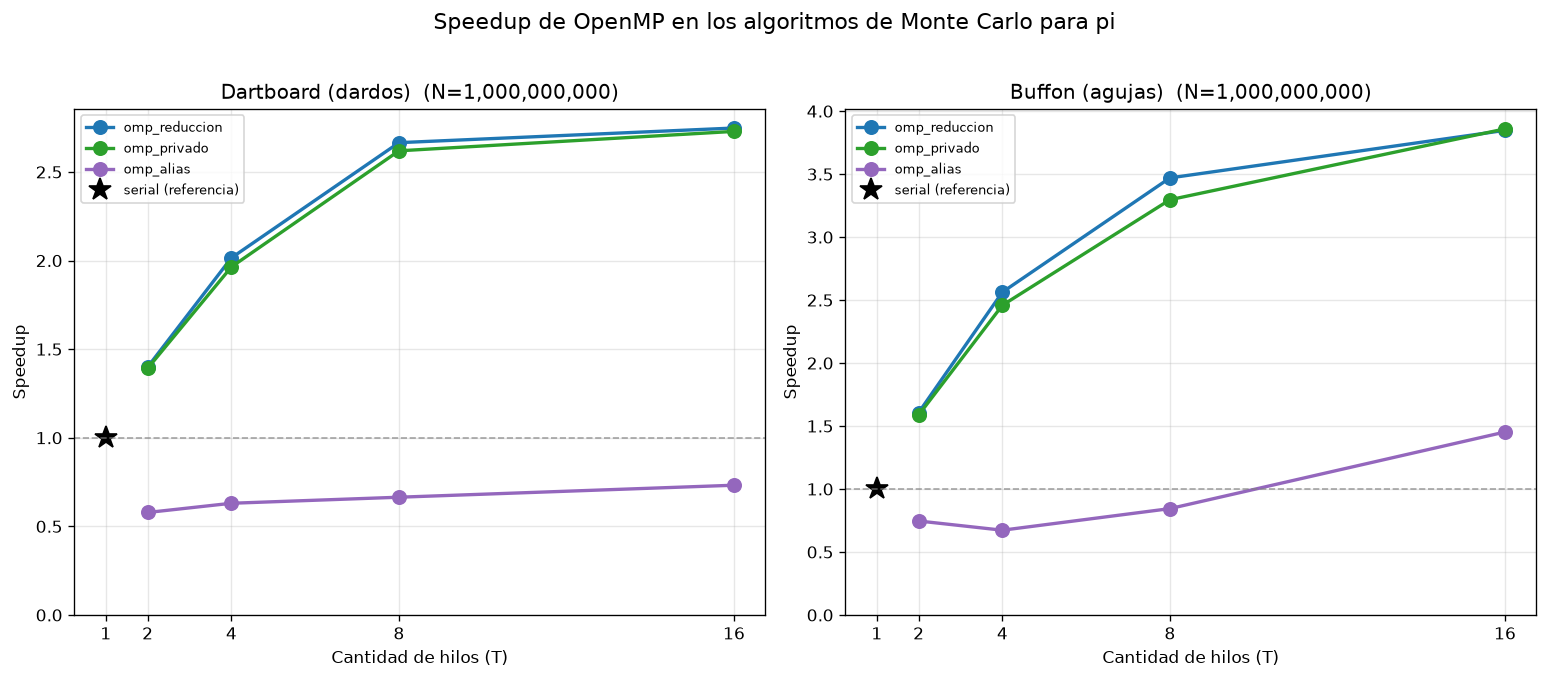
\includegraphics[width=0.98\textwidth]{figuras/speedup_montecarlo.png}
\caption{Speedup frente al número de hilos. Se observa que la variante con el estado del generador en puntero compartido (\texttt{omp\_alias}) no escala: es más lenta que la versión serial.}
\label{fig:speedup}
\end{figure}

\begin{figure}[ht]
\centering
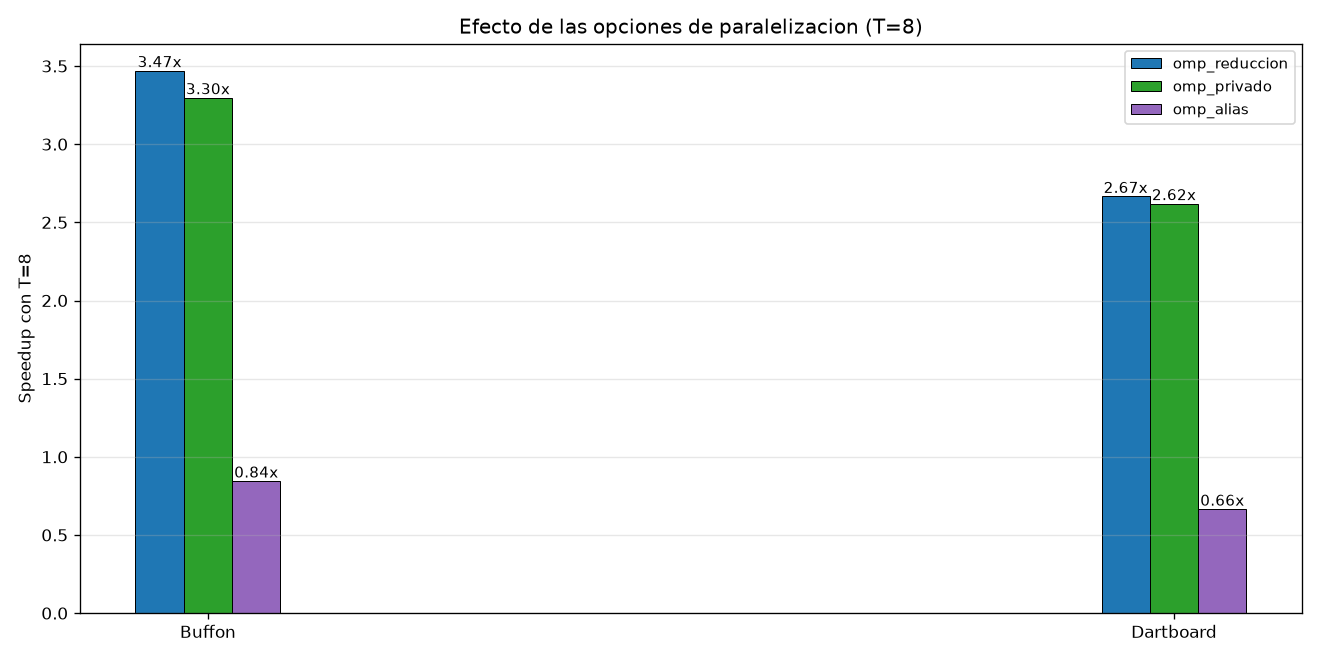
\includegraphics[width=0.85\textwidth]{figuras/escalamiento_algoritmos.png}
\caption{Efecto de cada opción de paralelización con $T = 8$. \texttt{omp\_alias} no solo escala peor, sino que empeora el tiempo respecto de la versión serial.}
\label{fig:variantes}
\end{figure}

\subsection{Costo por muestra}

\begin{figure}[ht]
\centering
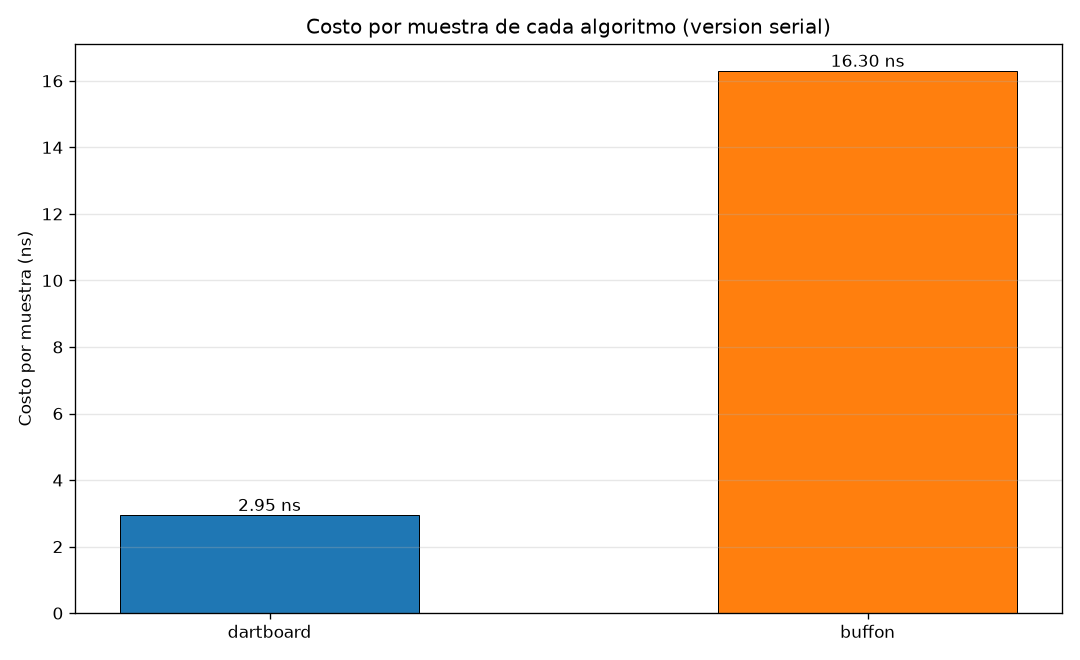
\includegraphics[width=0.75\textwidth]{figuras/costo_por_muestra.png}
\caption{Costo por muestra de cada algoritmo en la versión serial.}
\label{fig:costo}
\end{figure}

Con $N = 10^9$, el dartboard tarda 2.953\,s (2.95\,ns por muestra) y Buffon 16.305\,s (16.30\,ns por muestra). Buffon es \textbf{5.5 veces más caro por muestra}.

\subsection{Benchmark entre las dos máquinas}

\textit{[Pendiente de completar con la segunda máquina. La tabla y la gráfica quedan listas para ser rellenadas con los resultados del segundo equipo.]}

La tabla~\ref{tab:benchmark-maquinas} y la figura~\ref{fig:benchmark-maquinas} se llenan con la salida de \texttt{experiments/bench\_montecarlo.sh} ejecutado en cada equipo.

\begin{table}[ht]
\centering
\small
\begin{tabular}{|l|l|r|r|r|r|r|}
\hline
\textbf{Algoritmo} & \textbf{Máquina} & \textbf{N} & \textbf{T\_opt} & \textbf{tiempo (s)} & \textbf{ns/muestra} & \textbf{speedup} \\
\hline
dartboard & A & $10^9$ & \textit{(completar)} & & & \\
dartboard & B & $10^9$ & \textit{(completar)} & & & \\
buffon & A & $10^9$ & \textit{(completar)} & & & \\
buffon & B & $10^9$ & \textit{(completar)} & & & \\
\hline
\end{tabular}
\caption{Benchmark entre las dos máquinas. La comparación se hace con el mínimo de las repeticiones, igual que en el barrido de desempeño.}
\label{tab:benchmark-maquinas}
\end{table}

\begin{figure}[ht]
\centering
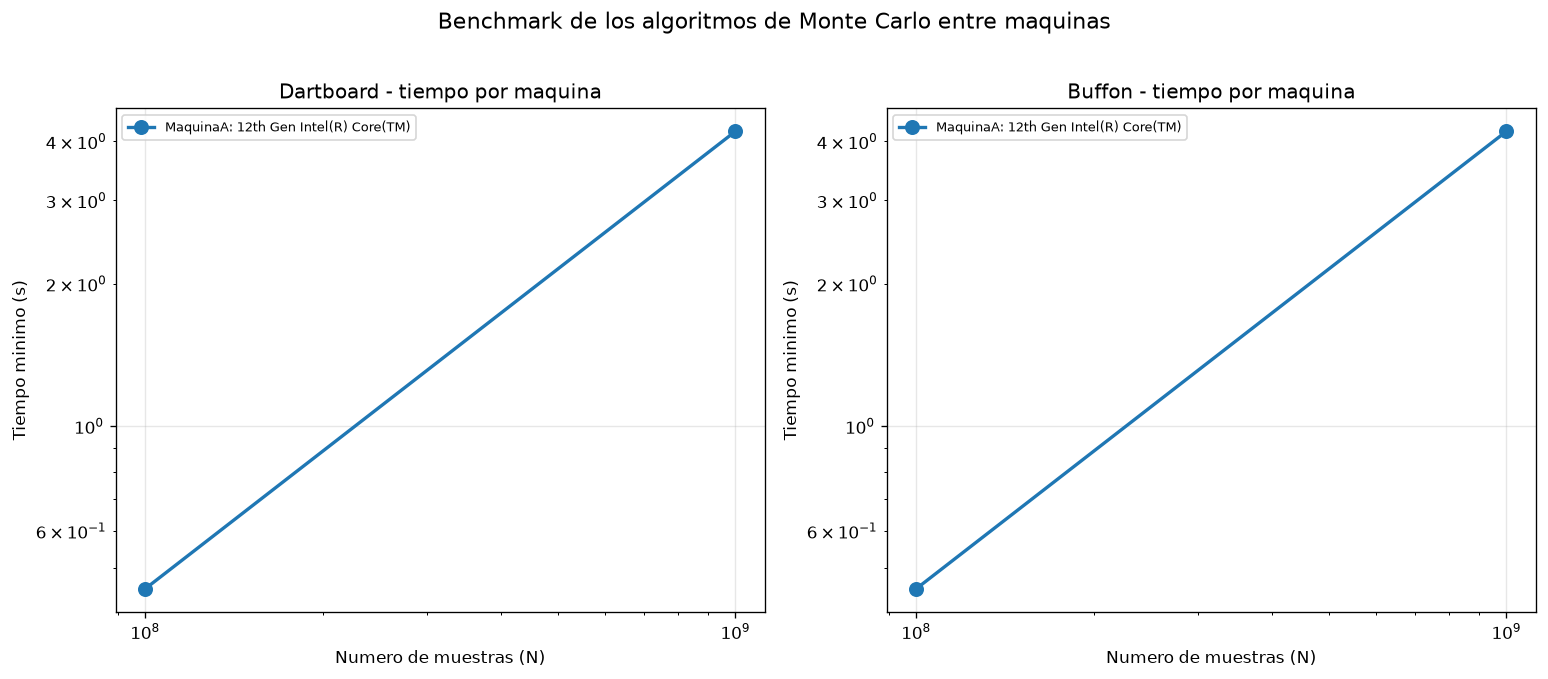
\includegraphics[width=0.95\textwidth]{figuras/benchmark_maquinas.png}
\caption{Tiempo mínimo de cada máquina para cada algoritmo y tamaño de muestra.}
\label{fig:benchmark-maquinas}
\end{figure}

\section{Análisis de resultados}

\subsection{El cuello de botella es el generador de números aleatorios, no la aritmética}

El perfilado de CPU (tabla~\ref{tab:gprof}) muestra que \texttt{rng\_double} ocupa más de la mitad del tiempo muestreado en ambos algoritmos, y el conteo de llamadas confirma que se invocan dos veces por muestra (una por cada coordenada). La aritmética del algoritmo, en cambio, es marginal: el predicado del dartboard es un producto y una suma.

Esto invierte la intuición habitual. En una aplicación de álgebra densa se esperaría que el costo dominante estuviera en las operaciones de coma flotante, y ahí es donde la paralelización rinde. Aquí el trabajo numérico es tan trivial (65 instrucciones por muestra en el dartboard) que lo que domina es la \emph{generación de los datos de entrada}. De ahí se siguen dos consecuencias:

\begin{enumerate}
    \item La paralelización funciona bien, porque el generador es \emph{encadenado}: cada muestra consume el estado anterior, así que no se puede paralelizar dentro de una muestra, pero sí entre muestras.
    \item El diseño del paralelismo debe centrarse en el generador, no en la aritmética: darle a cada hilo su propio estado es la decisión crítica.
\end{enumerate}

\subsection{Por qué el dartboard es 5.5 veces más rápido que Buffon}

La diferencia de costo por muestra (2.95\,ns frente a 16.30\,ns) tiene dos componentes, ambos medidos:

\begin{itemize}
    \item \textbf{El \texttt{sin} de Buffon.} El perfil de GProf atribuye al bucle de Buffon un 18.62\% del tiempo muestreado, frente al 8.26\% del dartboard, para una estructura de bucle idéntica. Esa diferencia de unos diez puntos es el costo de evaluar $\sin\theta$ en cada muestra. El dartboard no necesita ninguna función transcendentral.
    \item \textbf{El doble de instrucciones.} El dartboard ejecuta 65 instrucciones por muestra y Buffon 136, es decir, algo más del doble. La mayor parte de esa diferencia es la implementación de \texttt{sin}.
\end{itemize}

Esta es una consecuencia directa de la elección del modelo matemático, no de la implementación: el método del dartboard simplemente no necesita trigonometría.

\subsection{Por qué el dartboard también es más preciso}

La desviación teórica es $\sigma_{\text{dart}} = 1.642/\sqrt{N}$ para el dartboard y $\sigma_{\text{buff}} = 2.374/\sqrt{N}$ para Buffon, es decir, Buffon necesita unas 2.09 veces más muestras para la misma precisión.

Esto es relevante para el uso práctico del algoritmo: si se necesita $\pi$ con una tolerancia dada, el dartboard alcanza el objetivo con menos trabajo, y como además cada muestra es más barata, la ventaja combinada es de unas 11 veces menos tiempo para la misma exactitud.

\subsection{Por qué OpenMP escala bien aquí y mal en la multiplicación de matrices}

Este es el punto central del reto, y la respuesta está en el perfilado de memoria.

En el caso de estudio 2, la multiplicación de matrices tenía un conjunto de trabajo de 192\,MB por proceso y una tasa de fallo de caché L1 del 22.4\%. Al paralelizar, los hilos compiten por una jerarquía de caché que ya estaba saturada, y el speedup se quedaba en 3--4.5$\times$.

Aquí el cuadro es el opuesto: la tabla~\ref{tab:cachegrind} muestra una tasa de fallo de L1 del \textbf{0.0\%} en ambos algoritmos. El estado del generador son 32 bytes por hilo y el contador ocupa una línea de caché; en total, menos de 64 bytes de estado mutable por hilo. Todo el conjunto de trabajo cabe en la L1 del núcleo, y los hilos no compiten por nada.

La consecuencia directa se ve en las curvas de escalamiento: Buffon alcanza 3.85$\times$ con 16 hilos en un equipo de 12 hilos lógicos, y el dartboard 2.75$\times$. Son valores de escalamiento \emph{altos} comparados con el 3.11$\times$ del pthreads manual sobre multiplicación de matrices en el mismo equipo, y además el trabajo es mucho más simple.

La comparación de las dos tasas de fallo de caché es, por sí sola, la explicación de por qué el paralelismo rinde de forma tan distinta en los dos casos de estudio.

\subsection{Por qué el dartboard escala peor que Buffon, siendo más rápido}

Un resultado que parece contradictorio: el dartboard es 5.5 veces más rápido pero escala peor (2.75$\times$ contra 3.85$\times$).

La explicación es que el trabajo por muestra es tan pequeño (2.95\,ns) que los costos \emph{fijos} del paralelismo pesan proporcionalmente más. Con $T = 2$ el dartboard solo consigue 1.40$\times$ mientras Buffon consigue 1.61$\times$. A $N = 10^9$ la versión serial del dartboard tarda 2.95\,s, y una fracción de ese tiempo corresponde a gastos que no se paralelizan (arranque del equipo de hilos, sincronización final, planificación).

En otras palabras: \textbf{cuanto más barato es el trabajo por muestra, más overhead relativo hay en el paralelismo}. Es la misma razón por la que los algoritmos de la familia 1 en el caso de estudio 1 rendían mucho mejor con problemas grandes: el overhead se amortiza con más trabajo.

\subsection{El efecto del aliasing: la explicación del problema más importante}

La tabla~\ref{tab:speedup} muestra que la variante \texttt{omp\_alias}, que en realidad es la más natural de escribir, \textbf{es más lenta que la versión serial}: entre 0.58$\times$ y 0.73$\times$ en el dartboard. Lejos de acelerar el programa, la paralelización lo ralentiza.

La causa no está en OpenMP ni en el hardware, sino en el compilador. Cuando el estado del generador se accede como \texttt{rngs[tid]}, el compilador no puede demostrar que las escrituras a través de ese puntero no solapan con el acumulador de aciertos, así que mantiene el acumulador en memoria y lo recarga en cada iteración. El coste de esa recarga anula por completo la ganancia del paralelismo.

La solución, copiar el estado del generador a una variable local del hilo, es de una línea, y el efecto es de \textbf{3.8 veces} en el caso del dartboard y \textbf{2.6 veces} en el de Buffon.

La lección general es que \textbf{paralelizar no es solo escribir la directiva}: hay que asegurarse de que el compilador pueda mantener el estado de cada hilo en registros. Un paralelismo correcto en su lógica puede ser nulo en la práctica si el compilador no puede optimizar el bucle interno.

\subsection{El estado del generador y el determinismo}

Las versiones paralelas no producen exactamente el mismo resultado que la serial, y eso no es un defecto sino una decisión. La sección 3 explicó el porqué: obligar a que las dos versiones generen los mismos números obligaría a pre-generar las $N$ muestras en un arreglo, es decir, a pasar de un conjunto de trabajo de unos pocos bytes a uno de $O(N)$.

La tabla~\ref{tab:validacion} muestra que la diferencia no afecta la corrección: las medias de 20 corridas de la versión serial y de la paralela están ambas dentro de $0.4\sigma$ del valor real, y sus dispersiones coinciden con la teórica. La equivalencia es estadística, que es la que corresponde a un método estocástico.

\subsection{Qué queda por explicar: el benchmark entre máquinas}

\textit{[Pendiente de completar con la segunda máquina. El análisis de la comparación se completará cuando estén los datos del segundo equipo.]}

Lo que sí puede anticiparse con los datos de la máquina A es que el orden de los algoritmos y el orden de las variantes no deberían cambiar: la diferencia entre dartboard y Buffon (5.5$\times$) y el efecto del aliasing (3.8$\times$) son propiedades de la \emph{implementación}, no del hardware. Lo que sí depende del equipo es la \emph{forma} de las curvas de escalamiento, es decir, hasta qué cantidad de hilos rinde el paralelismo, que depende de la cantidad de núcleos físicos y de la jerarquía de caché.

\section{Conclusiones}

\subsection{Hallazgos}

\begin{enumerate}
    \item \textbf{El generador de números aleatorios es el cuello de botella, no la aritmética}. GProf atribuye más de la mitad del tiempo muestreado a \texttt{rng\_double} en ambos algoritmos. Esto invierte la intuición de las aplicaciones de álgebra densa y explica por qué el paralelismo rinde bien: el trabajo por muestra es independiente, solo el generador es compartido.

    \item \textbf{El dartboard domina a Buffon en las dos dimensiones}. Es 5.5 veces más rápido por muestra (2.95\,ns contra 16.30\,ns, con 65 instrucciones contra 136) porque no necesita evaluar $\sin\theta$, y además es un estimador más preciso: su desviación típica es $1.642/\sqrt{N}$ contra $2.374/\sqrt{N}$, es decir, Buffon necesita unas 2.09 veces más muestras para la misma exactitud.

    \item \textbf{El perfilado de memoria explica el cambio de comportamiento respecto del caso de estudio 2}. Con una tasa de fallo de caché L1 del 0.0\% frente al 22.4\% de la multiplicación de matrices, el conjunto de trabajo cabe en la L1 y los hilos no compiten por la caché. Por eso aquí el paralelismo escala mucho mejor: 3.85$\times$ con Buffon en un equipo de 12 hilos lógicos.

    \item \textbf{El trabajo más barato por muestra escala peor}. El dartboard, con 2.95\,ns por muestra, consigue solo 1.40$\times$ con dos hilos, mientras Buffon consigue 1.61$\times$. Los costos fijos del paralelismo pesan proporcionalmente más cuando el trabajo es más barato.

    \item \textbf{Un paralelismo correcto en su lógica puede ser nulo en la práctica}. La variante que accede al estado del generador a través de un puntero compartido resulta ser más lenta que la versión serial (0.58--0.73$\times$), porque el compilador no puede demostrar que el acumulador no se solapa con ese estado y lo mantiene en memoria en cada iteración. Copiar el estado a una variable local del hilo recupera un factor de 3.8$\times$ en el dartboard y 2.6$\times$ en Buffon.

    \item \textbf{La validación de efectividad de un método estocástico es por convergencia, no por igualdad}. Con 20 repeticiones por configuración, todas las medias están a menos de $0.4\sigma$ teóricas del valor real de $\pi$, y las dispersiones medidas coinciden con las previstas por la teoría del error.
\end{enumerate}

\subsection{Limitaciones}

\begin{itemize}
    \item El benchmark entre las dos máquinas quedó pendiente de completarse con los datos del segundo equipo; la comparación entre máquinas del enunciado está por tanto incompleta.
    \item Las mediciones de desempeño se realizaron con otros procesos ejecutándose en el equipo (navegador y herramientas de desarrollo), lo que resta precisión. Se reportan los \emph{mínimos} de 10 repeticiones precisamente para reducir el efecto del ruido del sistema, pero un equipo en reposo daría cifras ligeramente mejores.
    \item GProf es un perfilador por muestreo y su cobertura es parcial: con la instrumentación de \texttt{-pg} el tiempo real de la corrida fue de 21.9\,s para Buffon con $N=10^9$, de los cuales solo 3.44\,s quedaron atribuidos a muestras, porque el overhead de la propia instrumentación no se muestrea. Los porcentajes de GProf son por tanto proporciones del tiempo muestreado, y las cifras absolutas de costo por muestra del documento provienen de mediciones directas con \texttt{clock\_gettime}.
    \item Se implementaron cuatro variantes de paralelización de un conjunto mayor de opciones posibles. Por ejemplo, no se exploraron las variantes con partición dinámica del trabajo, ni la vectorización manual del predicado del dartboard con instrucciones SIMD, que exigiría desacoplar la generación de números aleatorios del test.
    \item El perfilado con Cachegrind usa $N = 10^7$ en lugar de $10^9$, por el costo de la simulación. La tasa de fallo es una propiedad del patrón de acceso y no debería variar con $N$, pero no se verificó para los tamaños mayores.
\end{itemize}

\subsection{Trabajo futuro}

\begin{itemize}
    \item Completar el benchmark entre las dos máquinas y extenderlo a más equipos para caracterizar el comportamiento del paralelismo en función de la cantidad de núcleos físicos y de la jerarquía de caché.
    \item Combinar la reducción privada con un \emph{schedule} balanceado dinámicamente, que es lo que la literatura de OpenMP muestra como óptimo cuando el trabajo por iteración es desigual.
    \item Vectorizar el predicado del dartboard: si se genera un bloque de números aleatorios con un generador SIMD-friendly y se acumulan cuatro resultados booleanos a la vez, el predicado podría evaluarse con instrucciones vectoriales. Es la vía para cerrar la diferencia de costo con Buffon.
    \item Evaluar el estimador de Buffon con la extensión de Laplace (dos rejillas de líneas perpendiculares), que reduce el número de lanzamientos necesarios para una precisión dada.
\end{itemize}

\section{Referencias}

\begin{itemize}
    \item \textbf{Buffon, G.-L. (1777)} --- \textit{Essai sur la théorie de la probabilité}. Formulación original del problema de la aguja. Referencia secundaria en \texttt{Buffon's needle problem}, Wikipedia.

    \item \textbf{Jörg Arndt y Christoph Haenel} --- \textit{Pi -- Unleashed: Exploring the infinite}, Springer. Capitulado 1, pág. 39: método del dartboard para la estimación de $\pi$, con implementación de referencia en C. Disponible en \texttt{books.google.com}.

    \item \textbf{Blackman, D. y Vigna, S.} --- \textit{Scrambled Linear Pseudorandom Number Generators}, ACM Transactions on Mathematical Software, 47(4), 2021. Referencia del generador \texttt{xoshiro256**} y del mezclador \texttt{SplitMix64} empleados.

    \item \textbf{OpenMP Application Programming Interface Examples, Version 6.0.1 (noviembre 2025)} --- ejemplos oficiales de la API OpenMP. Secciones 3.1 (\texttt{ploop.1.c}), 3.8 (\texttt{collapse.1.c}) y 5.3.5 (\texttt{task\_dep.5.c}) utilizados en el análisis de opciones de paralelización.

    \item \textbf{OpenMP Application Programming Interface Specification, Version 6.0 (noviembre 2024)} --- definición de las directivas, cláusulas \texttt{reduction}, \texttt{schedule} y \texttt{num\_threads}, y de la semántica de las variables compartidas y privadas.

    \item \textbf{GNU \texttt{gprof}} --- perfilador por muestreo con instrumentación en tiempo de compilación (\texttt{-pg}). Manual en \texttt{sourceware.org/binutils/docs}.

    \item \textbf{Valgrind: \texttt{cachegrind}} --- simulador de caché del proyecto Valgrind. Documentación en \texttt{valgrind.org/docs/manual/cg-manual.html}.

    \item \textbf{POSIX.1-2017 (IEEE Std 1003.1-2017)} --- \texttt{clock\_gettime}, \texttt{getrusage}, \texttt{rand\_r}, \texttt{drand48}. Especificación de la API POSIX utilizada para la medición del tiempo y de la memoria residente.

    \item \textbf{Intel\textsuperscript{\textregistered} 64 and IA-32 Architectures Software Developer's Manual, Volume 2} --- modelo de caché jerárquica, líneas de caché y concepto de \emph{false sharing}.

    \item \textbf{Brendan Gregg --- \textit{Systems Performance}} y su blog \texttt{brendangregg.com} --- referencias sobre las herramientas de línea de comandos para rendimiento en Linux y sobre el uso del mínimo de las repeticiones como estimador robusto frente al ruido del sistema.

    \item \textbf{Material del curso de Computación de Alto Rendimiento} --- presentaciones y grabaciones de clase (OpenMP, benchmark, profiling) utilizadas como referencia conceptual durante el desarrollo del reto.
\end{itemize}


\end{document}
